\documentclass[12pt,a4paper]{ctexart}
\usepackage{graphicx}
\usepackage{wrapfig}
\usepackage{float}
\usepackage{siunitx}
\usepackage{subfigure}
\usepackage{caption}
\usepackage{natbib}
\usepackage{listings} % 引入listings宏包用于插入代码
\usepackage{xcolor} % 引入xcolor宏包以支持更多的颜色设置

% 设置Verilog代码样式
\lstdefinestyle{verilog}{
    language=Verilog, % 设置语言为Verilog
    basicstyle=\small\ttfamily, % 设置基本字体样式
    keywordstyle=\color{blue}, % 关键字颜色设置
    commentstyle=\color{gray}\ttfamily, % 注释颜色和样式设置
    stringstyle=\color{red!60!black},
    numbers=left, % 行号在左边显示
    numberstyle=\tiny,
    frame=single, % 添加单线框
    rulecolor=\color{black!30}, % 边框颜色
    breaklines=true, % 允许自动换行
}

\title{实验 7:高速缓存 Cache}
\author{张子康 \ PB22020660}
\date{\today}

\begin{document}
\maketitle
\newpage
\section{实验目的与内容}
\subsection{实验目的}
在本次实验中,我们将学习高速缓存 Cache 的组织结构和工作机理。
\subsection{实验内容}
\subsubsection{任务 1:二路组相连 Cache}
根据给出的直接映射 Cache 的代码,实现二路组相连 Cache,支持 LRU 替换策略,通过助教提供的读写测试。
\subsubsection{任务 2:多样化的替换策略}
让你的 Cache 支持伪随机替换策略,FIFO 替换策略等除了 LRU 之外至少两种替换策略,通过助教提供的读写测试。
\subsubsection{任务 3:N 路组相连 Cache}
实现参数化的 N 路组相连 Cache,支持 LRU 替换策略
,通过助教提供的读写测试。
\section{逻辑设计}
本次实验中实现的高速缓存Cache均为N路组相连,故任务1与任务3实现代码相同。
\subsection{N路组相连Cache(LRU)}
\begin{lstlisting}[style=verilog]
module cache_lru #(
    parameter INDEX_WIDTH       = 3,    // Cache索引位宽 2^3=8行
    parameter LINE_OFFSET_WIDTH = 2,    // 行偏移位宽,决定了一行的宽度 2^2=4字
    parameter SPACE_OFFSET      = 2,    // 一个地址空间占1个字节,因此一个字需要4个地址空间,由于假设为整字读取,处理地址的时候可以默认后两位为0
    parameter WAY_NUM           = 2,    // Cache N路组相联(N=1的时候是直接映射),
    parameter N = 1                     // log_2(WAY_NUM),即2的N次方
)(
    input                     clk,    
    input                     rstn,
    /* CPU接口 */  
    input [31:0]              addr,   // CPU地址
    input                     r_req,  // CPU读请求
    input                     w_req,  // CPU写请求
    input [31:0]              w_data,  // CPU写数据
    output [31:0]             r_data,  // CPU读数据
    output reg                miss,   // 缓存未命中
    /* 内存接口 */  
    output reg                     mem_r,  // 内存读请求
    output reg                     mem_w,  // 内存写请求
    output reg [31:0]              mem_addr,  // 内存地址
    output reg [127:0] mem_w_data,  // 内存写数据 一次写一行
    input      [127:0] mem_r_data,  // 内存读数据 一次读一行
    input                          mem_ready  // 内存就绪信号
);

    // Cache参数
    localparam
        // Cache行宽度
        LINE_WIDTH = 32 << LINE_OFFSET_WIDTH,
        // 标记位宽度
        TAG_WIDTH = 32 - INDEX_WIDTH - LINE_OFFSET_WIDTH - SPACE_OFFSET,
        // Cache行数
        SET_NUM   = 1 << INDEX_WIDTH;
    
    // Cache相关寄存器
    reg [31:0]           addr_buf;    // 请求地址缓存-用于保留CPU请求地址
    reg [31:0]           w_data_buf;  // 写数据缓存
    reg op_buf;  // 读写操作缓存,用于在MISS状态下判断是读还是写,如果是写则需要将数据写回内存 0:读 1:写
    reg [LINE_WIDTH-1:0] ret_buf;     // 返回数据缓存-用于保留内存返回数据

    // Cache导线
    wire [INDEX_WIDTH-1:0] r_index;  // 索引读地址
    wire [INDEX_WIDTH-1:0] w_index;  // 索引写地址
    wire [LINE_WIDTH-1:0]  r_line;   // Data Bram读数据
    wire [LINE_WIDTH-1:0]  w_line;   // Data Bram写数据
    wire [LINE_WIDTH-1:0]  w_line_mask;  // Data Bram写数据掩码
    wire [LINE_WIDTH-1:0]  w_data_line;  // 输入写数据移位后的数据
    wire [TAG_WIDTH-1:0]   tag;      // CPU请求地址中分离的标记 用于比较 也可用于写入
    wire [TAG_WIDTH-1:0]   r_tag;    // Tag Bram读数据 用于比较
    wire [LINE_OFFSET_WIDTH-1:0] word_offset;  // 字偏移
    reg  [31:0]            cache_data;  // Cache数据
    reg  [31:0]            mem_data;    // 内存数据
    wire [31:0]            dirty_mem_addr; // 通过读出的tag和对应的index,偏移等得到脏块对应的内存地址并写回到正确的位置
    wire valid;  // Cache有效位
    wire dirty;  // Cache脏位.
    reg  w_valid;  // Cache写有效位
    reg  w_dirty;  // Cache写脏位
    wire hit;    // Cache命中

    // Cache相关控制信号
    reg addr_buf_we;  // 请求地址缓存写使能
    reg ret_buf_we;   // 返回数据缓存写使能
    reg [WAY_NUM-1:0]data_we;      // Cache写使能
    reg [WAY_NUM-1:0]tag_we;       // Cache标记写使能
    reg data_from_mem;  // 从内存读取数据
    reg refill;       // 标记需要重新填充,在MISS状态下接受到内存数据后置1,在IDLE状态下进行填充后置0

    // 状态机信号
    localparam 
        IDLE      = 3'd0,  // 空闲状态
        READ      = 3'd1,  // 读状态
        MISS      = 3'd2,  // 缺失时等待主存读出新块
        WRITE     = 3'd3,  // 写状态
        W_DIRTY   = 3'd4;  // 写缺失时等待主存写入脏块
    reg [2:0] CS;  // 状态机当前状态
    reg [2:0] NS;  // 状态机下一状态

    // 状态机
    always @(posedge clk or negedge rstn) begin
        if (!rstn) begin
            CS <= IDLE;
        end else begin
            CS <= NS;
        end
    end


    // 中间寄存器保留初始的请求地址和写数据,可以理解为addr_buf中的地址为当前Cache正在处理的请求地址,而addr中的地址为新的请求地址
    always @(posedge clk or negedge rstn) begin
        if (!rstn) begin
            addr_buf <= 0;
            ret_buf <= 0;
            w_data_buf <= 0;
            op_buf <= 0;
            refill <= 0;
        end else begin
            if (addr_buf_we) begin
                addr_buf <= addr;
                w_data_buf <= w_data;
                op_buf <= w_req;
            end
            if (ret_buf_we) begin
                ret_buf <= mem_r_data;
            end
            if (CS == MISS && mem_ready) begin
                refill <= 1;
            end
            if (CS == IDLE) begin
                refill <= 0;
            end
        end
    end

    // 对输入地址进行解码
    assign r_index = addr[INDEX_WIDTH+LINE_OFFSET_WIDTH+SPACE_OFFSET - 1: LINE_OFFSET_WIDTH+SPACE_OFFSET];
    assign w_index = addr_buf[INDEX_WIDTH+LINE_OFFSET_WIDTH+SPACE_OFFSET - 1: LINE_OFFSET_WIDTH+SPACE_OFFSET];
    assign tag = addr_buf[31:INDEX_WIDTH+LINE_OFFSET_WIDTH+SPACE_OFFSET];
    assign word_offset = addr_buf[LINE_OFFSET_WIDTH+SPACE_OFFSET-1:SPACE_OFFSET];

    // 脏块地址计算
    assign dirty_mem_addr = {r_tag, w_index}<<(LINE_OFFSET_WIDTH+SPACE_OFFSET);

    // 写回地址、数据寄存器
    reg [31:0] dirty_mem_addr_buf;
    reg [127:0] dirty_mem_data_buf;
    always @(posedge clk or negedge rstn) begin
        if (!rstn) begin
            dirty_mem_addr_buf <= 0;
            dirty_mem_data_buf <= 0;
        end else begin
            if (CS == READ || CS == WRITE) begin
                dirty_mem_addr_buf <= dirty_mem_addr;
                dirty_mem_data_buf <= r_line;
            end
        end
    end

    // 伪LRU
    reg [N-1:0] p;
    wire [N-1:0] r_p;
    reg p_we;

    wire valid_[WAY_NUM-1:0];  // Cache有效位
    wire dirty_[WAY_NUM-1:0];  // Cache脏位.
    reg  w_valid_[WAY_NUM-1:0];  // Cache写有效位
    reg  w_dirty_[WAY_NUM-1:0];  // Cache写脏位
    wire hit_[WAY_NUM-1:0];    // Cache命中
    wire [TAG_WIDTH-1:0] r_tag_[WAY_NUM-1:0];
    wire [LINE_WIDTH-1:0] w_line_[WAY_NUM-1:0];
    wire [LINE_WIDTH-1:0] r_line_[WAY_NUM-1:0];


    // 生成相关块
    // 伪LRU
    reg [(WAY_NUM-2>0?WAY_NUM-2:0):0] age;
    wire [(WAY_NUM-2>0?WAY_NUM-2:0):0] r_age;
    reg age_we;
    bram #(
            .ADDR_WIDTH(INDEX_WIDTH),
            .DATA_WIDTH((WAY_NUM-2>0?WAY_NUM-2:0)+1) 
    ) bram_age(
            .clk(clk),
            .raddr(r_index),
            .waddr(w_index),
            .din(age),
            .we(age_we),
            .dout(r_age)
    );

    generate
        genvar i;
        for (i = 0; i<WAY_NUM; i=i+1) begin:Bram
            // Tag Bram
            bram #(
                .ADDR_WIDTH(INDEX_WIDTH),
                .DATA_WIDTH(TAG_WIDTH + 2) // 最高位为有效位,次高位为脏位,低位为标记位
            ) tag_bram(
                .clk(clk),
                .raddr(r_index),
                .waddr(w_index),
                .din({w_valid,w_dirty, tag}),
                .we(tag_we[i]),
                .dout({valid_[i],dirty_[i], r_tag_[i]})
            );
            // Data Bram
            bram #(
                .ADDR_WIDTH(INDEX_WIDTH),
                .DATA_WIDTH(LINE_WIDTH)
            ) data_bram(
                .clk(clk),
                .raddr(r_index),
                .waddr(w_index),
                .din(w_line),
                .we(data_we[i]),
                .dout(r_line_[i])
            );
        end
    endgenerate


    // 判定Cache是否命中
    reg [N-1:0] j,tem_j,tem_j2,tem_j3,i_,tem_i;
    reg flag,tem;
    integer i1;    
    initial begin
        flag=0;
        tem=0;
        j=0;
        tem_j=0;  
        i_=0;
        tem_i=0;
    end
    always @(*) begin
        if(CS==READ || CS==WRITE)begin
            flag=0;
            tem=0;
            j=0;
            tem_j=0;
            i_=0;
            tem_i=0;
            // 若命中j中为命中的块的序号
            for (i1 = 0;i1<WAY_NUM ; i1=i1+1) begin
                tem=flag;
                flag=tem || (r_tag_[i1] == tag && valid_[i1]);
                if(r_tag_[i1] == tag && valid_[i1])begin
                    j=i1;
                end
            end
            // 若未命中,则计算需要替换的块的序号,存在j中
            if(!flag)begin
                for(i1=0;i1<N;i1=i1+1)begin
                    tem_j=j;
                    j=(tem_j<<1)+r_age[i_];
                    tem_i=i_;
                    i_=((tem_i+1)<<1)-r_age[tem_i];
                end
            end 
        end
    end
    assign r_tag=r_tag_[j];
    assign dirty=dirty_[j];
    assign r_line=r_line_[j];
    assign hit = flag;

    // 写入Cache 这里要判断是命中后写入还是未命中后写入
    assign w_line_mask = 32'hFFFFFFFF << (word_offset*32);   // 写入数据掩码
    assign w_data_line = w_data_buf << (word_offset*32);     // 写入数据移位
    assign w_line = (CS == IDLE && op_buf) ? ret_buf & ~w_line_mask | w_data_line : // 写入未命中,需要将内存数据与写入数据合并
                    (CS == IDLE) ? ret_buf : // 读取未命中
                    r_line & ~w_line_mask | w_data_line; // 写入命中,需要对读取的数据与写入的数据进行合并

    // 选择输出数据 从Cache或者从内存 这里的选择与行大小有关,因此如果你调整了行偏移位宽,这里也需要调整
    always @(*) begin
        case (word_offset)
            0: begin
                cache_data = r_line[31:0];
                mem_data = ret_buf[31:0];
            end
            1: begin
                cache_data = r_line[63:32];
                mem_data = ret_buf[63:32];
            end
            2: begin
                cache_data = r_line[95:64];
                mem_data = ret_buf[95:64];
            end
            3: begin
                cache_data = r_line[127:96];
                mem_data = ret_buf[127:96];
            end
            default: begin
                cache_data = 0;
                mem_data = 0;
            end
        endcase
    end

    assign r_data = data_from_mem ? mem_data : hit ? cache_data : 0;

    // 状态机更新逻辑
    always @(*) begin
        case(CS)
            IDLE: begin
                if (r_req) begin
                    NS = READ;
                end else if (w_req) begin
                    NS = WRITE;
                end else begin
                    NS = IDLE;
                end
            end
            READ: begin
                if (miss&& !dirty) begin
                    NS = MISS;
                end else if (miss && dirty) begin
                    NS = W_DIRTY;
                end else if (r_req) begin
                    NS = READ;
                end else if (w_req) begin
                    NS = WRITE;
                end else begin
                    NS = IDLE;
                end
            end
            MISS: begin
                if (mem_ready) begin // 这里回到IDLE的原因是为了延迟一周期,等待主存读出的新块写入Cache中的对应位置
                    NS = IDLE;
                end else begin
                    NS = MISS;
                end
            end
            WRITE: begin
                if (miss && !dirty) begin
                    NS = MISS;
                end else if (miss && dirty) begin
                    NS = W_DIRTY;
                end else if (r_req) begin
                    NS = READ;
                end else if (w_req) begin
                    NS = WRITE;
                end else begin
                    NS = IDLE;
                end
            end
            W_DIRTY: begin
                if (mem_ready) begin  // 写完脏块后回到MISS状态等待主存读出新块
                    NS = MISS;
                end else begin
                    NS = W_DIRTY;
                end
            end
            default: begin
                NS = IDLE;
            end
        endcase
    end
    initial begin
        p=0;
    end
    // 状态机控制信号
    always @(*) begin
        addr_buf_we   = 1'b0;
        ret_buf_we    = 1'b0;
        data_we       = 0;
        tag_we        = 0;
        w_valid       = 1'b0;
        w_dirty       = 1'b0;
        data_from_mem = 1'b0;
        miss          = 1'b0;
        mem_r         = 1'b0;
        mem_w         = 1'b0;
        mem_addr      = 32'b0;
        mem_w_data    = 0;
        tem_j2=0;
        tem_j3=0;
        age_we=0;
        case(CS)
            IDLE: begin
                addr_buf_we = 1'b1; // 请求地址缓存写使能
                miss = 1'b0;
                ret_buf_we = 1'b0;
                if(refill) begin
                    data_from_mem = 1'b1;
                    w_valid = 1'b1;
                    w_dirty = 1'b0;
                    data_we = 1'b1<<j;
                    tag_we = 1'b1<<j;
                    if (op_buf) begin // 写
                        w_dirty = 1'b1;
                    end 
                    // 更新age
                    age_we=1;
                    age=r_age;
                    for (i1 = 0;i1< N;i1=i1+1) begin
                        age[tem_j3]=~j[i1];
                        tem_j3=tem_j2;
                        tem_j2=((tem_j3+1)<<1)-j[i1];
                    end
                end
            end
            READ: begin
                data_from_mem = 1'b0;
                if (hit) begin // 命中
                    miss = 1'b0;
                    addr_buf_we = 1'b1; // 请求地址缓存写使能
                    // 更新age
                    age_we=1;
                    age=r_age;
                    for (i1 = 0;i1< N;i1=i1+1) begin
                        age[tem_j3]=~j[i1];
                        tem_j3=tem_j2;
                        tem_j2=((tem_j3+1)<<1)-j[i1];
                    end
                end else begin // 未命中
                    miss = 1'b1;
                    addr_buf_we = 1'b0; 
                    if (dirty) begin // 脏数据需要写回
                        mem_w = 1'b1;
                        mem_addr = dirty_mem_addr;
                        mem_w_data = r_line; // 写回数据
                    end
                end
            end
            MISS: begin
                miss = 1'b1;
                mem_r = 1'b1;
                mem_addr = addr_buf;
                if (mem_ready) begin
                    mem_r = 1'b0;
                    ret_buf_we = 1'b1;
                end 
            end 
            WRITE: begin
                data_from_mem = 1'b0;
                if (hit) begin // 命中
                    miss = 1'b0;
                    addr_buf_we = 1'b1; // 请求地址缓存写使能
                    w_valid = 1'b1;
                    w_dirty = 1'b1;
                    // 通过控制写使能信号控制写入块的序号
                    data_we = 1'b1<<j;
                    tag_we = 1'b1<<j;
                    // 更新age
                    age_we=1;
                    age=r_age;
                    for (i1 = 0;i1< N;i1=i1+1) begin
                        age[tem_j3]=~j[i1];
                        tem_j3=tem_j2;
                        tem_j2=((tem_j3+1)<<1)-j[i1];
                    end
                end else begin // 未命中
                    miss = 1'b1;
                    addr_buf_we = 1'b0; 
                    if (dirty) begin // 脏数据需要写回
                        mem_w = 1'b1;
                        mem_addr = dirty_mem_addr;
                        mem_w_data = r_line; // 写回数据
                    end
                end
            end
            W_DIRTY: begin
                miss = 1'b1;
                mem_w = 1'b1;
                mem_addr = dirty_mem_addr_buf;
                mem_w_data = dirty_mem_data_buf;
                if (mem_ready) begin
                    mem_w = 1'b0;
                end
            end
            default:;
        endcase
    end

endmodule
\end{lstlisting}
采用伪LRU实现,具体原理如下:
\begin{figure}[H]
    \centering
    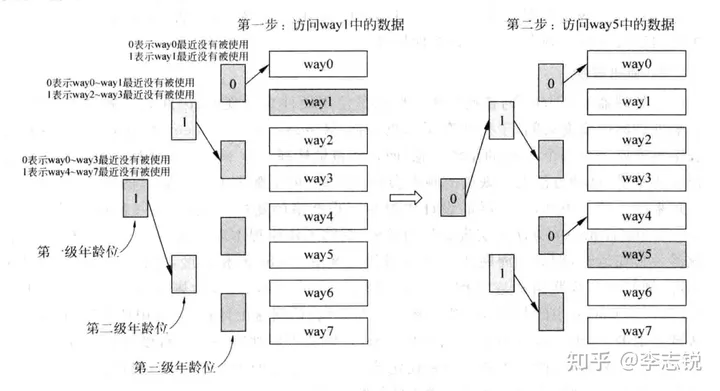
\includegraphics[scale=0.6]{lru.png}
\end{figure}
\subsection{多样化的替换策略}
主要通过更改j的计算方法实现。
\subsubsection{FIFO}
\begin{lstlisting}[style=verilog]
/*
直接映射Cache
- Cache行数:8行
- 块大小:4字(16字节 128位)
- 采用写回写分配策略
*/
module cache_fifo #(
    parameter INDEX_WIDTH       = 3,    // Cache索引位宽 2^3=8行
    parameter LINE_OFFSET_WIDTH = 2,    // 行偏移位宽,决定了一行的宽度 2^2=4字
    parameter SPACE_OFFSET      = 2,    // 一个地址空间占1个字节,因此一个字需要4个地址空间,由于假设为整字读取,处理地址的时候可以默认后两位为0
    parameter WAY_NUM           = 2,    // Cache N路组相联(N=1的时候是直接映射),
    parameter N = 1                     // log_2(WAY_NUM),即2的N次方
)(
    input                     clk,    
    input                     rstn,
    /* CPU接口 */  
    input [31:0]              addr,   // CPU地址
    input                     r_req,  // CPU读请求
    input                     w_req,  // CPU写请求
    input [31:0]              w_data,  // CPU写数据
    output [31:0]             r_data,  // CPU读数据
    output reg                miss,   // 缓存未命中
    /* 内存接口 */  
    output reg                     mem_r,  // 内存读请求
    output reg                     mem_w,  // 内存写请求
    output reg [31:0]              mem_addr,  // 内存地址
    output reg [127:0] mem_w_data,  // 内存写数据 一次写一行
    input      [127:0] mem_r_data,  // 内存读数据 一次读一行
    input                          mem_ready  // 内存就绪信号
);

    // Cache参数
    localparam
        // Cache行宽度
        LINE_WIDTH = 32 << LINE_OFFSET_WIDTH,
        // 标记位宽度
        TAG_WIDTH = 32 - INDEX_WIDTH - LINE_OFFSET_WIDTH - SPACE_OFFSET,
        // Cache行数
        SET_NUM   = 1 << INDEX_WIDTH;
    
    // Cache相关寄存器
    reg [31:0]           addr_buf;    // 请求地址缓存-用于保留CPU请求地址
    reg [31:0]           w_data_buf;  // 写数据缓存
    reg op_buf;  // 读写操作缓存,用于在MISS状态下判断是读还是写,如果是写则需要将数据写回内存 0:读 1:写
    reg [LINE_WIDTH-1:0] ret_buf;     // 返回数据缓存-用于保留内存返回数据

    // Cache导线
    wire [INDEX_WIDTH-1:0] r_index;  // 索引读地址
    wire [INDEX_WIDTH-1:0] w_index;  // 索引写地址
    wire [LINE_WIDTH-1:0]  r_line;   // Data Bram读数据
    wire [LINE_WIDTH-1:0]  w_line;   // Data Bram写数据
    wire [LINE_WIDTH-1:0]  w_line_mask;  // Data Bram写数据掩码
    wire [LINE_WIDTH-1:0]  w_data_line;  // 输入写数据移位后的数据
    wire [TAG_WIDTH-1:0]   tag;      // CPU请求地址中分离的标记 用于比较 也可用于写入
    wire [TAG_WIDTH-1:0]   r_tag;    // Tag Bram读数据 用于比较
    wire [LINE_OFFSET_WIDTH-1:0] word_offset;  // 字偏移
    reg  [31:0]            cache_data;  // Cache数据
    reg  [31:0]            mem_data;    // 内存数据
    wire [31:0]            dirty_mem_addr; // 通过读出的tag和对应的index,偏移等得到脏块对应的内存地址并写回到正确的位置
    wire valid;  // Cache有效位
    wire dirty;  // Cache脏位.
    reg  w_valid;  // Cache写有效位
    reg  w_dirty;  // Cache写脏位
    wire hit;    // Cache命中

    // Cache相关控制信号
    reg addr_buf_we;  // 请求地址缓存写使能
    reg ret_buf_we;   // 返回数据缓存写使能
    reg [WAY_NUM-1:0]data_we;      // Cache写使能
    reg [WAY_NUM-1:0]tag_we;       // Cache标记写使能
    reg data_from_mem;  // 从内存读取数据
    reg refill;       // 标记需要重新填充,在MISS状态下接受到内存数据后置1,在IDLE状态下进行填充后置0

    // 状态机信号
    localparam 
        IDLE      = 3'd0,  // 空闲状态
        READ      = 3'd1,  // 读状态
        MISS      = 3'd2,  // 缺失时等待主存读出新块
        WRITE     = 3'd3,  // 写状态
        W_DIRTY   = 3'd4;  // 写缺失时等待主存写入脏块
    reg [2:0] CS;  // 状态机当前状态
    reg [2:0] NS;  // 状态机下一状态

    // 状态机
    always @(posedge clk or negedge rstn) begin
        if (!rstn) begin
            CS <= IDLE;
        end else begin
            CS <= NS;
        end
    end

    // 中间寄存器保留初始的请求地址和写数据,可以理解为addr_buf中的地址为当前Cache正在处理的请求地址,而addr中的地址为新的请求地址
    always @(posedge clk or negedge rstn) begin
        if (!rstn) begin
            addr_buf <= 0;
            ret_buf <= 0;
            w_data_buf <= 0;
            op_buf <= 0;
            refill <= 0;
        end else begin
            if (addr_buf_we) begin
                addr_buf <= addr;
                w_data_buf <= w_data;
                op_buf <= w_req;
            end
            if (ret_buf_we) begin
                ret_buf <= mem_r_data;
            end
            if (CS == MISS && mem_ready) begin
                refill <= 1;
            end
            if (CS == IDLE) begin
                refill <= 0;
            end
        end
    end

    // 对输入地址进行解码
    assign r_index = addr[INDEX_WIDTH+LINE_OFFSET_WIDTH+SPACE_OFFSET - 1: LINE_OFFSET_WIDTH+SPACE_OFFSET];
    assign w_index = addr_buf[INDEX_WIDTH+LINE_OFFSET_WIDTH+SPACE_OFFSET - 1: LINE_OFFSET_WIDTH+SPACE_OFFSET];
    assign tag = addr_buf[31:INDEX_WIDTH+LINE_OFFSET_WIDTH+SPACE_OFFSET];
    assign word_offset = addr_buf[LINE_OFFSET_WIDTH+SPACE_OFFSET-1:SPACE_OFFSET];

    // 脏块地址计算
    assign dirty_mem_addr = {r_tag, w_index}<<(LINE_OFFSET_WIDTH+SPACE_OFFSET);

    // 写回地址、数据寄存器
    reg [31:0] dirty_mem_addr_buf;
    reg [127:0] dirty_mem_data_buf;
    always @(posedge clk or negedge rstn) begin
        if (!rstn) begin
            dirty_mem_addr_buf <= 0;
            dirty_mem_data_buf <= 0;
        end else begin
            if (CS == READ || CS == WRITE) begin
                dirty_mem_addr_buf <= dirty_mem_addr;
                dirty_mem_data_buf <= r_line;
            end
        end
    end

    // FIFO
    reg [N-1:0] p;
    wire [N-1:0] r_p;
    reg p_we;

    wire valid_[WAY_NUM-1:0];  // Cache有效位
    wire dirty_[WAY_NUM-1:0];  // Cache脏位.
    reg  w_valid_[WAY_NUM-1:0];  // Cache写有效位
    reg  w_dirty_[WAY_NUM-1:0];  // Cache写脏位
    wire hit_[WAY_NUM-1:0];    // Cache命中
    wire [TAG_WIDTH-1:0] r_tag_[WAY_NUM-1:0];
    wire [LINE_WIDTH-1:0] w_line_[WAY_NUM-1:0];
    wire [LINE_WIDTH-1:0] r_line_[WAY_NUM-1:0];

    // 该块用于存储要写入的块序号
    bram #(
            .ADDR_WIDTH(INDEX_WIDTH),
            .DATA_WIDTH(N) 
    ) bram_p(
            .clk(clk),
            .raddr(r_index),
            .waddr(w_index),
            .din(p),
            .we(p_we),
            .dout(r_p)
    );

    generate
        genvar i;
        for (i = 0; i<WAY_NUM; i=i+1) begin:Bram
            // Tag Bram
            bram #(
                .ADDR_WIDTH(INDEX_WIDTH),
                .DATA_WIDTH(TAG_WIDTH + 2) // 最高位为有效位,次高位为脏位,低位为标记位
            ) tag_bram(
                .clk(clk),
                .raddr(r_index),
                .waddr(w_index),
                .din({w_valid,w_dirty, tag}),
                .we(tag_we[i]),
                .dout({valid_[i],dirty_[i], r_tag_[i]})
            );
            // Data Bram
            bram #(
                .ADDR_WIDTH(INDEX_WIDTH),
                .DATA_WIDTH(LINE_WIDTH)
            ) data_bram(
                .clk(clk),
                .raddr(r_index),
                .waddr(w_index),
                .din(w_line),
                .we(data_we[i]),
                .dout(r_line_[i])
            );
        end
    endgenerate
    


    // 判定Cache是否命中
    reg [N-1:0] j,tem_j;
    reg flag,tem;
    integer i1;    
    initial begin
        flag=0;
        tem=0;
        j=6'b000000;
        tem_j=6'b000000;  
    end
    always @(*) begin
        if(CS==READ || CS==WRITE)begin
            flag=0;
            tem=0;
            j=6'b000000;
            tem_j=6'b000000;
            // 若命中则j为命中的块的序号
            for (i1 = 0;i1<WAY_NUM ; i1=i1+1) begin
                tem=flag;
                flag=tem || (r_tag_[i1] == tag && valid_[i1]);
                if(r_tag_[i1] == tag && valid_[i1])begin
                    j=i1;
                end
            end
            // 若未命中则j为需要写入的块的序号
            if(!flag)begin
                j=r_p;
            end 
        end
        
    end
    assign r_tag=r_tag_[j];
    assign dirty=dirty_[j];
    assign r_line=r_line_[j];
    assign hit = flag;

    // 写入Cache 这里要判断是命中后写入还是未命中后写入
    assign w_line_mask = 32'hFFFFFFFF << (word_offset*32);   // 写入数据掩码
    assign w_data_line = w_data_buf << (word_offset*32);     // 写入数据移位
    assign w_line = (CS == IDLE && op_buf) ? ret_buf & ~w_line_mask | w_data_line : // 写入未命中,需要将内存数据与写入数据合并
                    (CS == IDLE) ? ret_buf : // 读取未命中
                    r_line & ~w_line_mask | w_data_line; // 写入命中,需要对读取的数据与写入的数据进行合并

    // 选择输出数据 从Cache或者从内存 这里的选择与行大小有关,因此如果你调整了行偏移位宽,这里也需要调整
    always @(*) begin
        case (word_offset)
            0: begin
                cache_data = r_line[31:0];
                mem_data = ret_buf[31:0];
            end
            1: begin
                cache_data = r_line[63:32];
                mem_data = ret_buf[63:32];
            end
            2: begin
                cache_data = r_line[95:64];
                mem_data = ret_buf[95:64];
            end
            3: begin
                cache_data = r_line[127:96];
                mem_data = ret_buf[127:96];
            end
            default: begin
                cache_data = 0;
                mem_data = 0;
            end
        endcase
    end

    assign r_data = data_from_mem ? mem_data : hit ? cache_data : 0;

    // 状态机更新逻辑
    always @(*) begin
        case(CS)
            IDLE: begin
                if (r_req) begin
                    NS = READ;
                end else if (w_req) begin
                    NS = WRITE;
                end else begin
                    NS = IDLE;
                end
            end
            READ: begin
                if (miss&& !dirty) begin
                    NS = MISS;
                end else if (miss && dirty) begin
                    NS = W_DIRTY;
                end else if (r_req) begin
                    NS = READ;
                end else if (w_req) begin
                    NS = WRITE;
                end else begin
                    NS = IDLE;
                end
            end
            MISS: begin
                if (mem_ready) begin // 这里回到IDLE的原因是为了延迟一周期,等待主存读出的新块写入Cache中的对应位置
                    NS = IDLE;
                end else begin
                    NS = MISS;
                end
            end
            WRITE: begin
                if (miss && !dirty) begin
                    NS = MISS;
                end else if (miss && dirty) begin
                    NS = W_DIRTY;
                end else if (r_req) begin
                    NS = READ;
                end else if (w_req) begin
                    NS = WRITE;
                end else begin
                    NS = IDLE;
                end
            end
            W_DIRTY: begin
                if (mem_ready) begin  // 写完脏块后回到MISS状态等待主存读出新块
                    NS = MISS;
                end else begin
                    NS = W_DIRTY;
                end
            end
            default: begin
                NS = IDLE;
            end
        endcase
    end
    initial begin
        p=0;
    end
    // 状态机控制信号
    always @(*) begin
        addr_buf_we   = 1'b0;
        ret_buf_we    = 1'b0;
        data_we       = 0;
        tag_we        = 0;
        w_valid       = 1'b0;
        w_dirty       = 1'b0;
        data_from_mem = 1'b0;
        miss          = 1'b0;
        mem_r         = 1'b0;
        mem_w         = 1'b0;
        mem_addr      = 32'b0;
        mem_w_data    = 0;
        p=r_p;
        p_we=0;
        case(CS)
            IDLE: begin
                addr_buf_we = 1'b1; // 请求地址缓存写使能
                miss = 1'b0;
                ret_buf_we = 1'b0;
                if(refill) begin
                    data_from_mem = 1'b1;
                    w_valid = 1'b1;
                    w_dirty = 1'b0;
                    data_we = 1'b1<<j;
                    tag_we = 1'b1<<j;
                    // 块序号指针向后移动一位
                    p=r_p+1;
                    p_we=1;
                    if (op_buf) begin // 写
                        w_dirty = 1'b1;
                    end 
                end
            end
            READ: begin
                data_from_mem = 1'b0;
                if (hit) begin // 命中
                    miss = 1'b0;
                    addr_buf_we = 1'b1; // 请求地址缓存写使能
                end else begin // 未命中
                    miss = 1'b1;
                    addr_buf_we = 1'b0; 
                    if (dirty) begin // 脏数据需要写回
                        mem_w = 1'b1;
                        mem_addr = dirty_mem_addr;
                        mem_w_data = r_line; // 写回数据
                    end
                end
            end
            MISS: begin
                miss = 1'b1;
                mem_r = 1'b1;
                mem_addr = addr_buf;
                if (mem_ready) begin
                    mem_r = 1'b0;
                    ret_buf_we = 1'b1;
                end 
            end 
            WRITE: begin
                data_from_mem = 1'b0;
                if (hit) begin // 命中
                    miss = 1'b0;
                    addr_buf_we = 1'b1; // 请求地址缓存写使能
                    w_valid = 1'b1;
                    w_dirty = 1'b1;
                    data_we = 1'b1<<j;
                    tag_we = 1'b1<<j;
                end else begin // 未命中
                    miss = 1'b1;
                    addr_buf_we = 1'b0; 
                    if (dirty) begin // 脏数据需要写回
                        mem_w = 1'b1;
                        mem_addr = dirty_mem_addr;
                        mem_w_data = r_line; // 写回数据
                    end
                end
            end
            W_DIRTY: begin
                miss = 1'b1;
                mem_w = 1'b1;
                mem_addr = dirty_mem_addr_buf;
                mem_w_data = dirty_mem_data_buf;
                if (mem_ready) begin
                    mem_w = 1'b0;
                end
            end
            default:;
        endcase
    end

endmodule
\end{lstlisting}
\subsubsection{RANDOM}
采用伪随机数实现。
\begin{lstlisting}[style=verilog]
/*
直接映射Cache
- Cache行数:8行
- 块大小:4字(16字节 128位)
- 采用写回写分配策略
*/
module cache_random #(
    parameter INDEX_WIDTH       = 3,    // Cache索引位宽 2^3=8行
    parameter LINE_OFFSET_WIDTH = 2,    // 行偏移位宽,决定了一行的宽度 2^2=4字
    parameter SPACE_OFFSET      = 2,    // 一个地址空间占1个字节,因此一个字需要4个地址空间,由于假设为整字读取,处理地址的时候可以默认后两位为0
    parameter WAY_NUM           = 2,    // Cache N路组相联(N=1的时候是直接映射),
    parameter N = 0
)(
    input                     clk,    
    input                     rstn,
    /* CPU接口 */  
    input [31:0]              addr,   // CPU地址
    input                     r_req,  // CPU读请求
    input                     w_req,  // CPU写请求
    input [31:0]              w_data,  // CPU写数据
    output [31:0]             r_data,  // CPU读数据
    output reg                miss,   // 缓存未命中
    /* 内存接口 */  
    output reg                     mem_r,  // 内存读请求
    output reg                     mem_w,  // 内存写请求
    output reg [31:0]              mem_addr,  // 内存地址
    output reg [127:0] mem_w_data,  // 内存写数据 一次写一行
    input      [127:0] mem_r_data,  // 内存读数据 一次读一行
    input                          mem_ready  // 内存就绪信号
);

    // Cache参数
    localparam
        // Cache行宽度
        LINE_WIDTH = 32 << LINE_OFFSET_WIDTH,
        // 标记位宽度
        TAG_WIDTH = 32 - INDEX_WIDTH - LINE_OFFSET_WIDTH - SPACE_OFFSET,
        // Cache行数
        SET_NUM   = 1 << INDEX_WIDTH;
    
    // Cache相关寄存器
    reg [31:0]           addr_buf;    // 请求地址缓存-用于保留CPU请求地址
    reg [31:0]           w_data_buf;  // 写数据缓存
    reg op_buf;  // 读写操作缓存,用于在MISS状态下判断是读还是写,如果是写则需要将数据写回内存 0:读 1:写
    reg [LINE_WIDTH-1:0] ret_buf;     // 返回数据缓存-用于保留内存返回数据

    // Cache导线
    wire [INDEX_WIDTH-1:0] r_index;  // 索引读地址
    wire [INDEX_WIDTH-1:0] w_index;  // 索引写地址
    wire [LINE_WIDTH-1:0]  r_line;   // Data Bram读数据
    wire [LINE_WIDTH-1:0]  w_line;   // Data Bram写数据
    wire [LINE_WIDTH-1:0]  w_line_mask;  // Data Bram写数据掩码
    wire [LINE_WIDTH-1:0]  w_data_line;  // 输入写数据移位后的数据
    wire [TAG_WIDTH-1:0]   tag;      // CPU请求地址中分离的标记 用于比较 也可用于写入
    wire [TAG_WIDTH-1:0]   r_tag;    // Tag Bram读数据 用于比较
    wire [LINE_OFFSET_WIDTH-1:0] word_offset;  // 字偏移
    reg  [31:0]            cache_data;  // Cache数据
    reg  [31:0]            mem_data;    // 内存数据
    wire [31:0]            dirty_mem_addr; // 通过读出的tag和对应的index,偏移等得到脏块对应的内存地址并写回到正确的位置
    wire valid;  // Cache有效位
    wire dirty;  // Cache脏位.
    reg  w_valid;  // Cache写有效位
    reg  w_dirty;  // Cache写脏位
    wire hit;    // Cache命中

    // Cache相关控制信号
    reg addr_buf_we;  // 请求地址缓存写使能
    reg ret_buf_we;   // 返回数据缓存写使能
    reg [WAY_NUM-1:0]data_we;      // Cache写使能
    reg [WAY_NUM-1:0]tag_we;       // Cache标记写使能
    reg data_from_mem;  // 从内存读取数据
    reg refill;       // 标记需要重新填充,在MISS状态下接受到内存数据后置1,在IDLE状态下进行填充后置0

    // 状态机信号
    localparam 
        IDLE      = 3'd0,  // 空闲状态
        READ      = 3'd1,  // 读状态
        MISS      = 3'd2,  // 缺失时等待主存读出新块
        WRITE     = 3'd3,  // 写状态
        W_DIRTY   = 3'd4;  // 写缺失时等待主存写入脏块
    reg [2:0] CS;  // 状态机当前状态
    reg [2:0] NS;  // 状态机下一状态

    // 状态机
    always @(posedge clk or negedge rstn) begin
        if (!rstn) begin
            CS <= IDLE;
        end else begin
            CS <= NS;
        end
    end

    // 伪随机数
    reg [N-1:0] random;
    initial begin
        random=0;
    end
    always @(posedge clk) begin
        random<=random+1;
    end

    // 中间寄存器保留初始的请求地址和写数据,可以理解为addr_buf中的地址为当前Cache正在处理的请求地址,而addr中的地址为新的请求地址
    always @(posedge clk or negedge rstn) begin
        if (!rstn) begin
            addr_buf <= 0;
            ret_buf <= 0;
            w_data_buf <= 0;
            op_buf <= 0;
            refill <= 0;
        end else begin
            if (addr_buf_we) begin
                addr_buf <= addr;
                w_data_buf <= w_data;
                op_buf <= w_req;
            end
            if (ret_buf_we) begin
                ret_buf <= mem_r_data;
            end
            if (CS == MISS && mem_ready) begin
                refill <= 1;
            end
            if (CS == IDLE) begin
                refill <= 0;
            end
        end
    end

    // 对输入地址进行解码
    assign r_index = addr[INDEX_WIDTH+LINE_OFFSET_WIDTH+SPACE_OFFSET - 1: LINE_OFFSET_WIDTH+SPACE_OFFSET];
    assign w_index = addr_buf[INDEX_WIDTH+LINE_OFFSET_WIDTH+SPACE_OFFSET - 1: LINE_OFFSET_WIDTH+SPACE_OFFSET];
    assign tag = addr_buf[31:INDEX_WIDTH+LINE_OFFSET_WIDTH+SPACE_OFFSET];
    assign word_offset = addr_buf[LINE_OFFSET_WIDTH+SPACE_OFFSET-1:SPACE_OFFSET];

    // 脏块地址计算
    assign dirty_mem_addr = {r_tag, w_index}<<(LINE_OFFSET_WIDTH+SPACE_OFFSET);

    // 写回地址、数据寄存器
    reg [31:0] dirty_mem_addr_buf;
    reg [127:0] dirty_mem_data_buf;
    always @(posedge clk or negedge rstn) begin
        if (!rstn) begin
            dirty_mem_addr_buf <= 0;
            dirty_mem_data_buf <= 0;
        end else begin
            if (CS == READ || CS == WRITE) begin
                dirty_mem_addr_buf <= dirty_mem_addr;
                dirty_mem_data_buf <= r_line;
            end
        end
    end


    wire valid_[WAY_NUM-1:0];  // Cache有效位
    wire dirty_[WAY_NUM-1:0];  // Cache脏位.
    reg  w_valid_[WAY_NUM-1:0];  // Cache写有效位
    reg  w_dirty_[WAY_NUM-1:0];  // Cache写脏位
    wire hit_[WAY_NUM-1:0];    // Cache命中
    wire [TAG_WIDTH-1:0] r_tag_[WAY_NUM-1:0];
    wire [LINE_WIDTH-1:0] w_line_[WAY_NUM-1:0];
    wire [LINE_WIDTH-1:0] r_line_[WAY_NUM-1:0];

    generate
        genvar i;
        for (i = 0; i<WAY_NUM; i=i+1) begin:Bram
            // Tag Bram
            bram #(
                .ADDR_WIDTH(INDEX_WIDTH),
                .DATA_WIDTH(TAG_WIDTH + 2) // 最高位为有效位,次高位为脏位,低位为标记位
            ) tag_bram(
                .clk(clk),
                .raddr(r_index),
                .waddr(w_index),
                .din({w_valid,w_dirty, tag}),
                .we(tag_we[i]),
                .dout({valid_[i],dirty_[i], r_tag_[i]})
            );
            // Data Bram
            bram #(
                .ADDR_WIDTH(INDEX_WIDTH),
                .DATA_WIDTH(LINE_WIDTH)
            ) data_bram(
                .clk(clk),
                .raddr(r_index),
                .waddr(w_index),
                .din(w_line),
                .we(data_we[i]),
                .dout(r_line_[i])
            );
        end
    endgenerate
    


    // 判定Cache是否命中
    reg [N-1:0] j,tem_j;
    reg flag,tem;
    integer i1;    
    initial begin
        flag=0;
        tem=0;
        j=6'b000000;
        tem_j=6'b000000;  
    end
    always @(*) begin
        if(CS==READ || CS==WRITE)begin
            flag=0;
            tem=0;
            j=6'b000000;
            tem_j=6'b000000;
            for (i1 = 0;i1<WAY_NUM ; i1=i1+1) begin
                tem=flag;
                flag=tem || (r_tag_[i1] == tag && valid_[i1]);
                if(r_tag_[i1] == tag && valid_[i1])begin
                    j=i1;
                end
            end
            if(!flag)begin
                j=random;
            end 
        end
        
    end
    assign r_tag=r_tag_[j];
    assign dirty=dirty_[j];
    assign r_line=r_line_[j];
    assign hit = flag;

    // 写入Cache 这里要判断是命中后写入还是未命中后写入
    assign w_line_mask = 32'hFFFFFFFF << (word_offset*32);   // 写入数据掩码
    assign w_data_line = w_data_buf << (word_offset*32);     // 写入数据移位
    assign w_line = (CS == IDLE && op_buf) ? ret_buf & ~w_line_mask | w_data_line : // 写入未命中,需要将内存数据与写入数据合并
                    (CS == IDLE) ? ret_buf : // 读取未命中
                    r_line & ~w_line_mask | w_data_line; // 写入命中,需要对读取的数据与写入的数据进行合并

    // 选择输出数据 从Cache或者从内存 这里的选择与行大小有关,因此如果你调整了行偏移位宽,这里也需要调整
    always @(*) begin
        case (word_offset)
            0: begin
                cache_data = r_line[31:0];
                mem_data = ret_buf[31:0];
            end
            1: begin
                cache_data = r_line[63:32];
                mem_data = ret_buf[63:32];
            end
            2: begin
                cache_data = r_line[95:64];
                mem_data = ret_buf[95:64];
            end
            3: begin
                cache_data = r_line[127:96];
                mem_data = ret_buf[127:96];
            end
            default: begin
                cache_data = 0;
                mem_data = 0;
            end
        endcase
    end

    assign r_data = data_from_mem ? mem_data : hit ? cache_data : 0;

    // 状态机更新逻辑
    always @(*) begin
        case(CS)
            IDLE: begin
                if (r_req) begin
                    NS = READ;
                end else if (w_req) begin
                    NS = WRITE;
                end else begin
                    NS = IDLE;
                end
            end
            READ: begin
                if (miss&& !dirty) begin
                    NS = MISS;
                end else if (miss && dirty) begin
                    NS = W_DIRTY;
                end else if (r_req) begin
                    NS = READ;
                end else if (w_req) begin
                    NS = WRITE;
                end else begin
                    NS = IDLE;
                end
            end
            MISS: begin
                if (mem_ready) begin // 这里回到IDLE的原因是为了延迟一周期,等待主存读出的新块写入Cache中的对应位置
                    NS = IDLE;
                end else begin
                    NS = MISS;
                end
            end
            WRITE: begin
                if (miss && !dirty) begin
                    NS = MISS;
                end else if (miss && dirty) begin
                    NS = W_DIRTY;
                end else if (r_req) begin
                    NS = READ;
                end else if (w_req) begin
                    NS = WRITE;
                end else begin
                    NS = IDLE;
                end
            end
            W_DIRTY: begin
                if (mem_ready) begin  // 写完脏块后回到MISS状态等待主存读出新块
                    NS = MISS;
                end else begin
                    NS = W_DIRTY;
                end
            end
            default: begin
                NS = IDLE;
            end
        endcase
    end
    initial begin
        p=0;
    end
    // 状态机控制信号
    always @(*) begin
        addr_buf_we   = 1'b0;
        ret_buf_we    = 1'b0;
        data_we       = 0;
        tag_we        = 0;
        w_valid       = 1'b0;
        w_dirty       = 1'b0;
        data_from_mem = 1'b0;
        miss          = 1'b0;
        mem_r         = 1'b0;
        mem_w         = 1'b0;
        mem_addr      = 32'b0;
        mem_w_data    = 0;
        case(CS)
            IDLE: begin
                addr_buf_we = 1'b1; // 请求地址缓存写使能
                miss = 1'b0;
                ret_buf_we = 1'b0;
                if(refill) begin
                    data_from_mem = 1'b1;
                    w_valid = 1'b1;
                    w_dirty = 1'b0;
                    data_we = 1'b1<<j;
                    tag_we = 1'b1<<j;
                    if (op_buf) begin // 写
                        w_dirty = 1'b1;
                    end 
                end
            end
            READ: begin
                data_from_mem = 1'b0;
                if (hit) begin // 命中
                    miss = 1'b0;
                    addr_buf_we = 1'b1; // 请求地址缓存写使能
                end else begin // 未命中
                    miss = 1'b1;
                    addr_buf_we = 1'b0; 
                    if (dirty) begin // 脏数据需要写回
                        mem_w = 1'b1;
                        mem_addr = dirty_mem_addr;
                        mem_w_data = r_line; // 写回数据
                    end
                end
            end
            MISS: begin
                miss = 1'b1;
                mem_r = 1'b1;
                mem_addr = addr_buf;
                if (mem_ready) begin
                    mem_r = 1'b0;
                    ret_buf_we = 1'b1;
                end 
            end 
            WRITE: begin
                data_from_mem = 1'b0;
                if (hit) begin // 命中
                    miss = 1'b0;
                    addr_buf_we = 1'b1; // 请求地址缓存写使能
                    w_valid = 1'b1;
                    w_dirty = 1'b1;
                    data_we = 1'b1<<j;
                    tag_we = 1'b1<<j;
                end else begin // 未命中
                    miss = 1'b1;
                    addr_buf_we = 1'b0; 
                    if (dirty) begin // 脏数据需要写回
                        mem_w = 1'b1;
                        mem_addr = dirty_mem_addr;
                        mem_w_data = r_line; // 写回数据
                    end
                end
            end
            W_DIRTY: begin
                miss = 1'b1;
                mem_w = 1'b1;
                mem_addr = dirty_mem_addr_buf;
                mem_w_data = dirty_mem_data_buf;
                if (mem_ready) begin
                    mem_w = 1'b0;
                end
            end
            default:;
        endcase
    end

endmodule
\end{lstlisting}
\section{仿真结果与分析}
\subsection{N路组相连Cache(LRU)}
\begin{figure}[H]
    \centering
    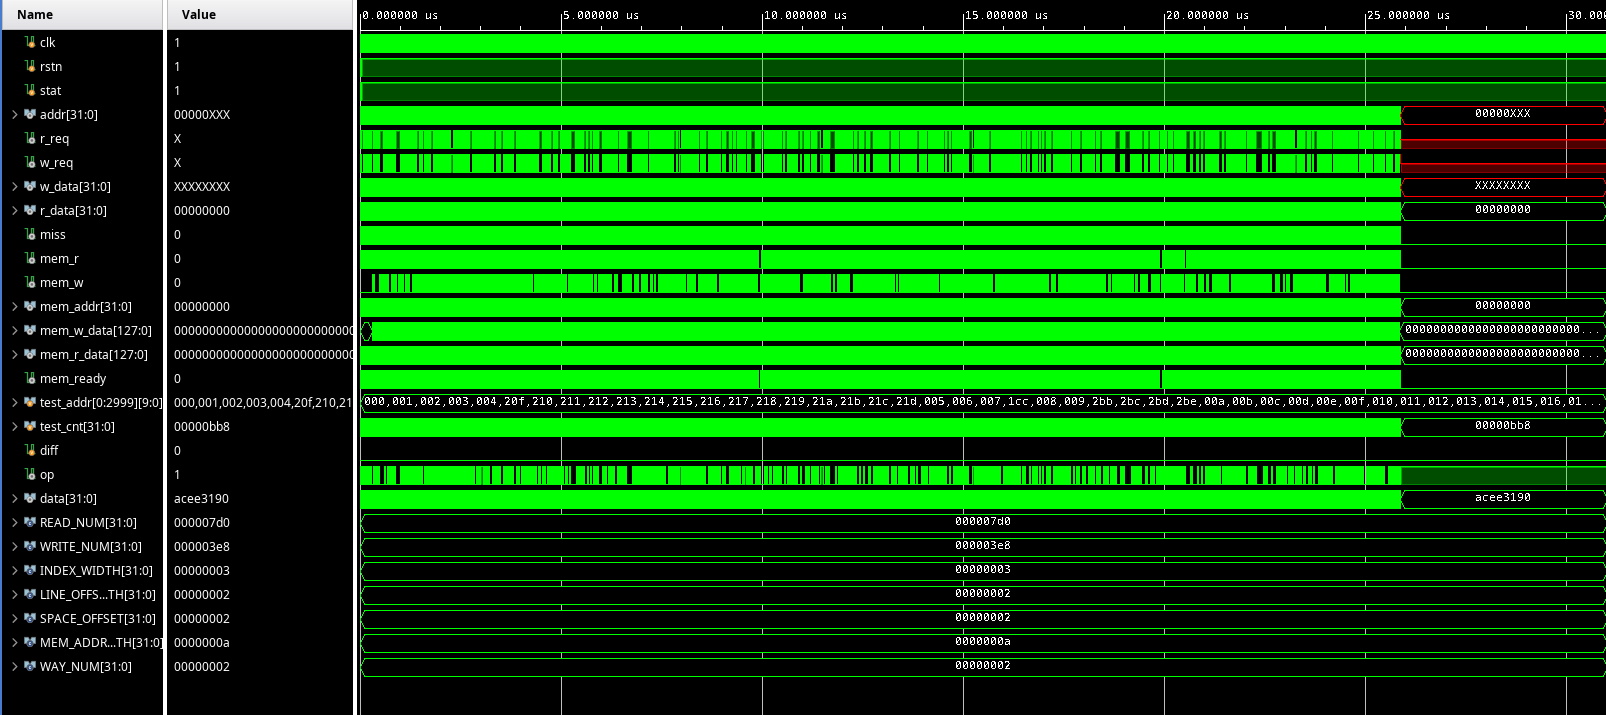
\includegraphics[scale=0.4]{pic/lru_2.png}
    \caption{2路组相连,采用伪LRU替换策略}
\end{figure}
\begin{figure}[H]
    \centering
    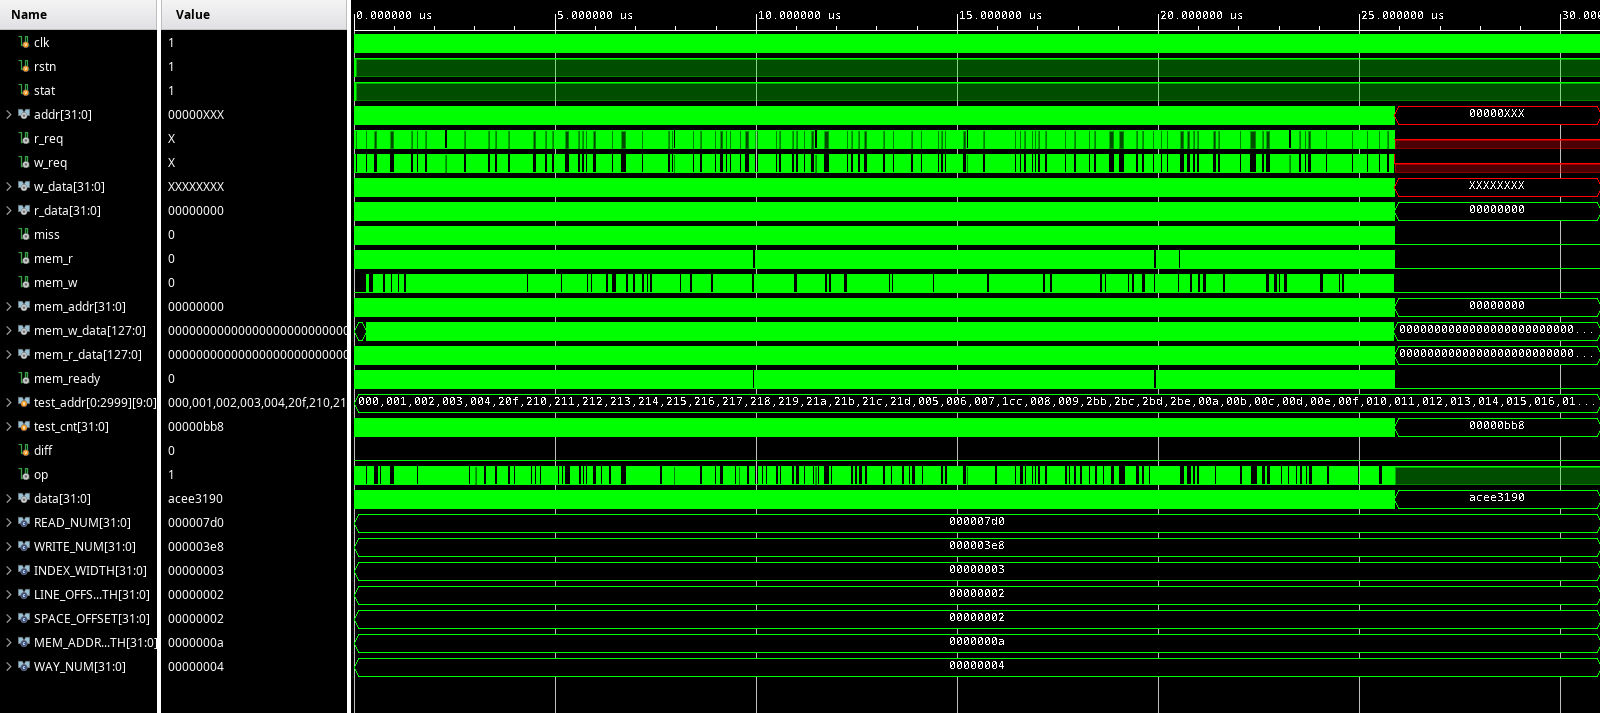
\includegraphics[scale=0.4]{pic/lru_4.png}
    \caption{4路组相连,采用伪LRU替换策略}
\end{figure}
\begin{figure}[H]
    \centering
    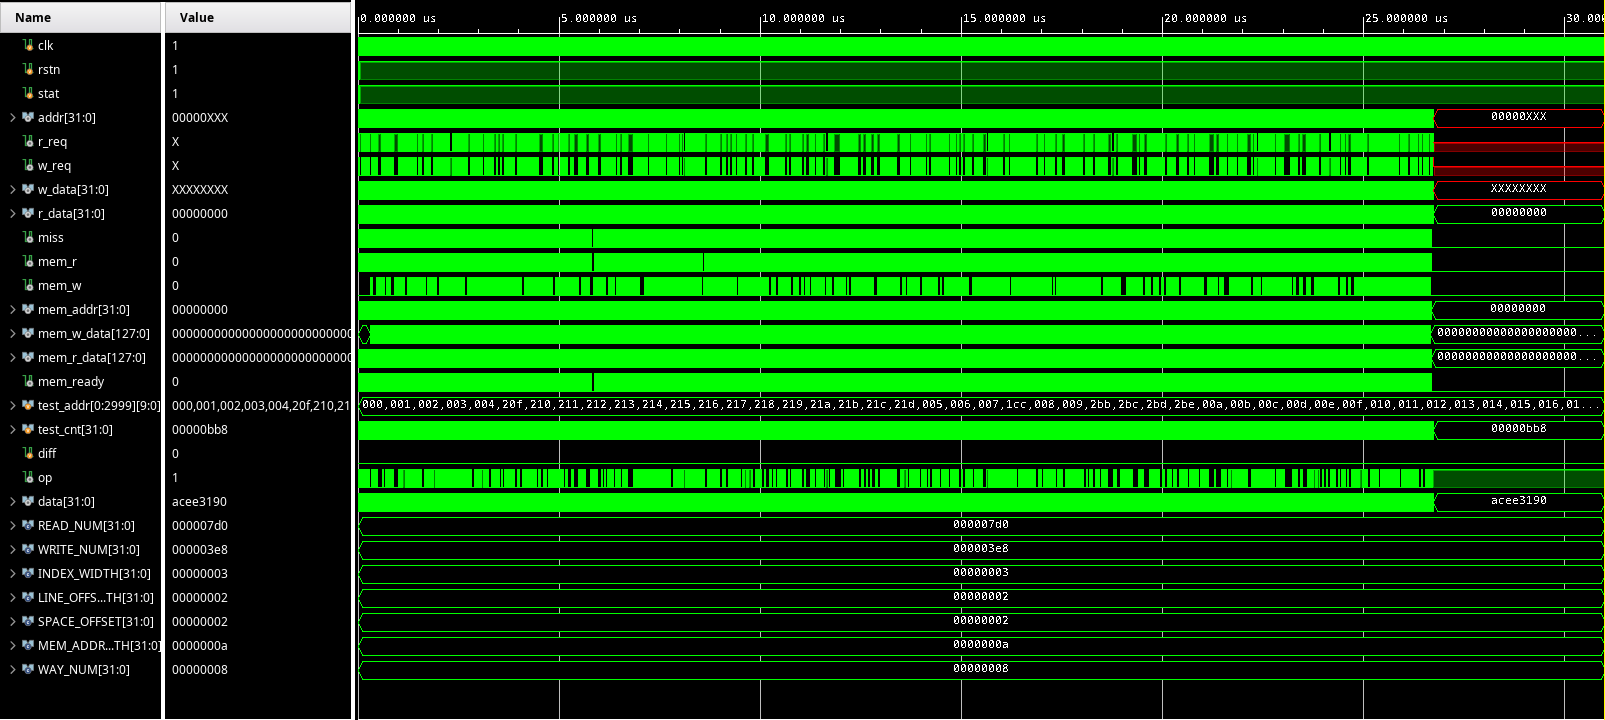
\includegraphics[scale=0.4]{pic/lru_8.png}
    \caption{8路组相连,采用伪LRU替换策略}
\end{figure}
\begin{figure}[H]
    \centering
    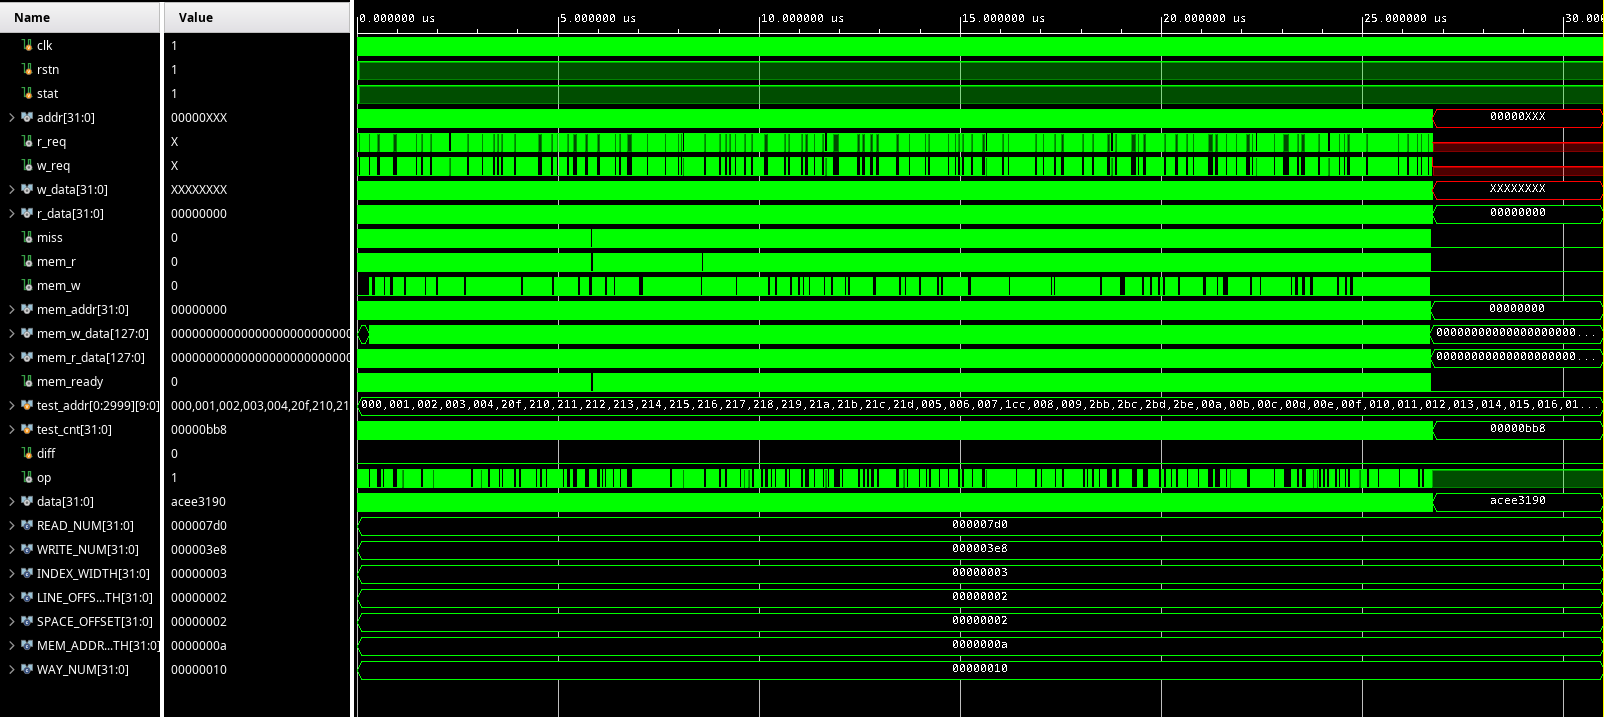
\includegraphics[scale=0.4]{pic/lru_16.png}
    \caption{16路组相连,采用伪LRU替换策略}
\end{figure}
\subsection{其他替换策略(FIFO,伪随机)}
\subsubsection{FIFO}
\begin{figure}[H]
    \centering
    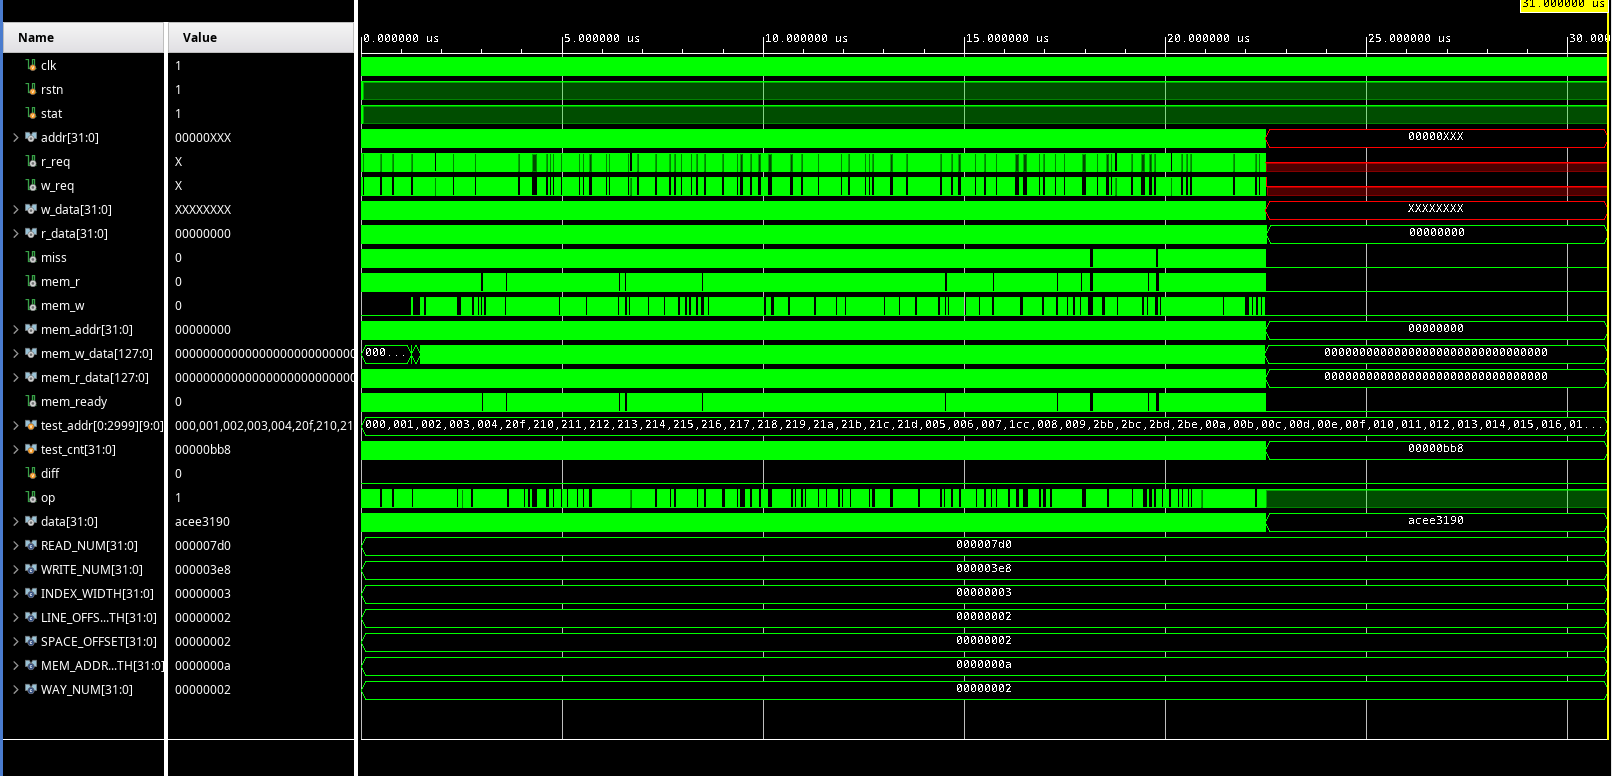
\includegraphics[scale=0.4]{pic/fifo.png}
    \caption{2路组相连,采用FIFO替换策略}
\end{figure}
\subsubsection{伪随机}
\begin{figure}[H]
    \centering
    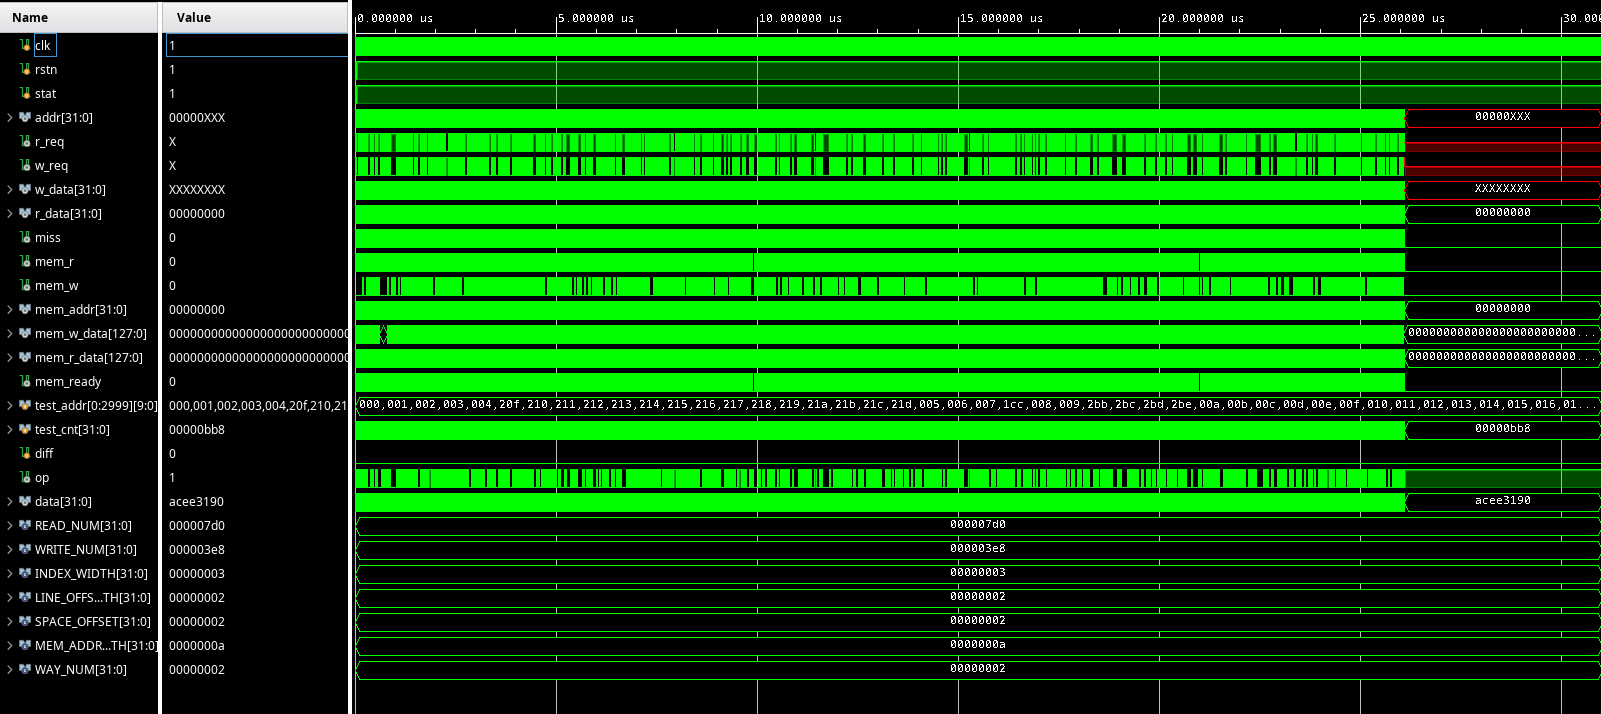
\includegraphics[scale=0.4]{pic/random.png}
    \caption{2路组相连,采用伪随机替换策略}
\end{figure}
\section{测试结果与分析}
从仿真中可以看到测试结果均正确(diff信号始终为0)
\section{总结}
本次实验实现了高速缓存Cache,采用的替换测略包括伪LRU(N路组相联)
,FIFO(2路组相连)和伪随机(2路组相连)。
\end{document}